\documentclass[nooutcomes]{ximera}
%% handout
%% space
%% newpage
%% numbers
%% nooutcomes

\usepackage{fullpage}
\newcommand{\RR}{\mathbb R}
\renewcommand{\d}{\,d}
\newcommand{\dd}[2][]{\frac{d #1}{d #2}}
\renewcommand{\l}{\ell}
\newcommand{\ddx}{\frac{d}{dx}}
\newcommand{\dfn}{\textbf}
\newcommand{\eval}[1]{\bigg[ #1 \bigg]}

\usepackage{multicol}

\renewenvironment{freeResponse}{
\ifhandout\setbox0\vbox\bgroup\else
\begin{trivlist}\item[\hskip \labelsep\bfseries Solution:\hspace{2ex}]
\fi}
{\ifhandout\egroup\else
\end{trivlist}
\fi} %% we can turn off input when making a master document

\title{4.9 Antiderivatives}  

\begin{document}
\begin{abstract}		\end{abstract}
\maketitle



%problem 1
\begin{problem}
Find the most general antiderivative of the function
$$ g(t) = e^{-2t} - 5 + 6\sqrt{t}-\frac{7}{t} + \frac{5}{11 + t^2} $$
		\begin{freeResponse}
		Note that:
			\begin{itemize}
			\item  taking an antiderivative is \dfn{linear} over addition, meaning that we can find the antiderivative of each term of $g(t)$, and then add them together.
			\item  An antiderivative of $e^{-2t}$ is $-\frac{1}{2} e^{-2t}$.
			\item  An antiderivative of $5$ is $5t$.
			\item  An antiderivative of $6 \sqrt{t}$ is $6 \left( \frac{2}{3} t^{\frac{3}{2}} \right) = 4t^{\frac{3}{2}}$.
			\item  An antiderivative of $\frac{7}{t}$ is $7 \ln |t|$.
			\item  An antiderivative of $\frac{5}{11 + t^2} = \frac{5}{11} \cdot \frac{1}{1 + \left( \frac{t}{\sqrt{11}} \right)^2 }$
			is $\frac{5}{\sqrt{11}} \arctan \left( \frac{t}{\sqrt{11}} \right)$
			\end{itemize}
		Thus, the most general anti-derivative of $g(t)$ is:
		$$ -\frac{1}{2} e^{-2t} - 5t + 4t^{\frac{3}{2}} - 7 \ln |t| + \frac{5}{\sqrt{11}} \arctan \left( \frac{t}{\sqrt{11}} \right) + C $$
		\end{freeResponse}
		
		
\end{problem}








%problem 2
\begin{problem}
Assume that $f^\prime (t) = 4t^3 + 2t$ and $f(3) = 5$.  Find $f(t)$.
		\begin{freeResponse}
		By taking the antiderivative of $f^\prime (t)$, we know that $f(t)$ is of the form
		$$f(t) = t^4 + t^2 + C .$$
		Then,
		$$ 5 = f(3) = 3^4 + 3^2 + C = 81 + 9 + C = 90 + C$$
		$$\Longrightarrow \quad  C = -85 $$
		and so
		$$ f(t) = t^4 + t^2 - 85. $$
		\end{freeResponse}
		
		
		

\end{problem}
	
	
	
	


%problem 3
\begin{problem}
  Given the graph of a function:
  \begin{image}
    \includegraphics[scale=.8]{"Figure 1".png}
  \end{image}
  
  \begin{enumerate}
    \item
      Sketch four anti-derivatives of the given function.
      \begin{freeResponse} \hfil
        \begin{image}
          \includegraphics[scale=.8]{"Figure 2".png}
        \end{image}
      \end{freeResponse}


    \item
      What is algebraic representation for the graph of given function $f$?
      \begin{freeResponse}
        $f(x) = x^2$
      \end{freeResponse}


    \item
      Using the function $f$ you found in part (b) and your sketches of the antiderivative in part (a), what is the algebraic representation of one of the anti-derivatives, $F$.
      \begin{freeResponse}
       The general antiderivative is $F(x) = \frac{1}{3}x^3+C$.  One particular antiderivative might be $F(x) = \frac{1}{3}x^3+2$
      \end{freeResponse}

    \item
      Suppose we're given $h(x) = (1/3)x^3$, what is $h'(x)$?
      \begin{freeResponse}
        $h'(x) = x^2$.
      \end{freeResponse}


    \item
      In the general case, what is the relationship between $f$, $F$, $h$, and $h'$?
      \begin{freeResponse}
        We have $F' = f = h'$ and $h = F-C$. In the particular case where we chose $C=2$, we have $h=F-2$.
      \end{freeResponse}
  \end{enumerate}
\end{problem}



%problem 4
\begin{problem}
	
Consider an object moving along a line with velocity $v(t)=\pi \sin(\pi t)$ on $[0,2]$ and initial position $s(0)=0$.  Time is measured in seconds and velocity in m/s.

\begin{enumerate}
	
	\item Determine the position function, $s(t)$, on $[0,2]$.
	
	\begin{freeResponse}	
		General antiderivative of $v(t)$: $s(t)=-\cos(\pi t)+C$\\
		Apply initial position: $s(t)=-\cos(\pi t)+C \implies 0=s(0)=-\cos(0)+C \implies C=1$\\
		Position function: $s(t)=-\cos(\pi t)+1$
	\end{freeResponse}
	
	\item Mark the position of the object at the time $t=1$ on the line below.
	  \begin{image}
    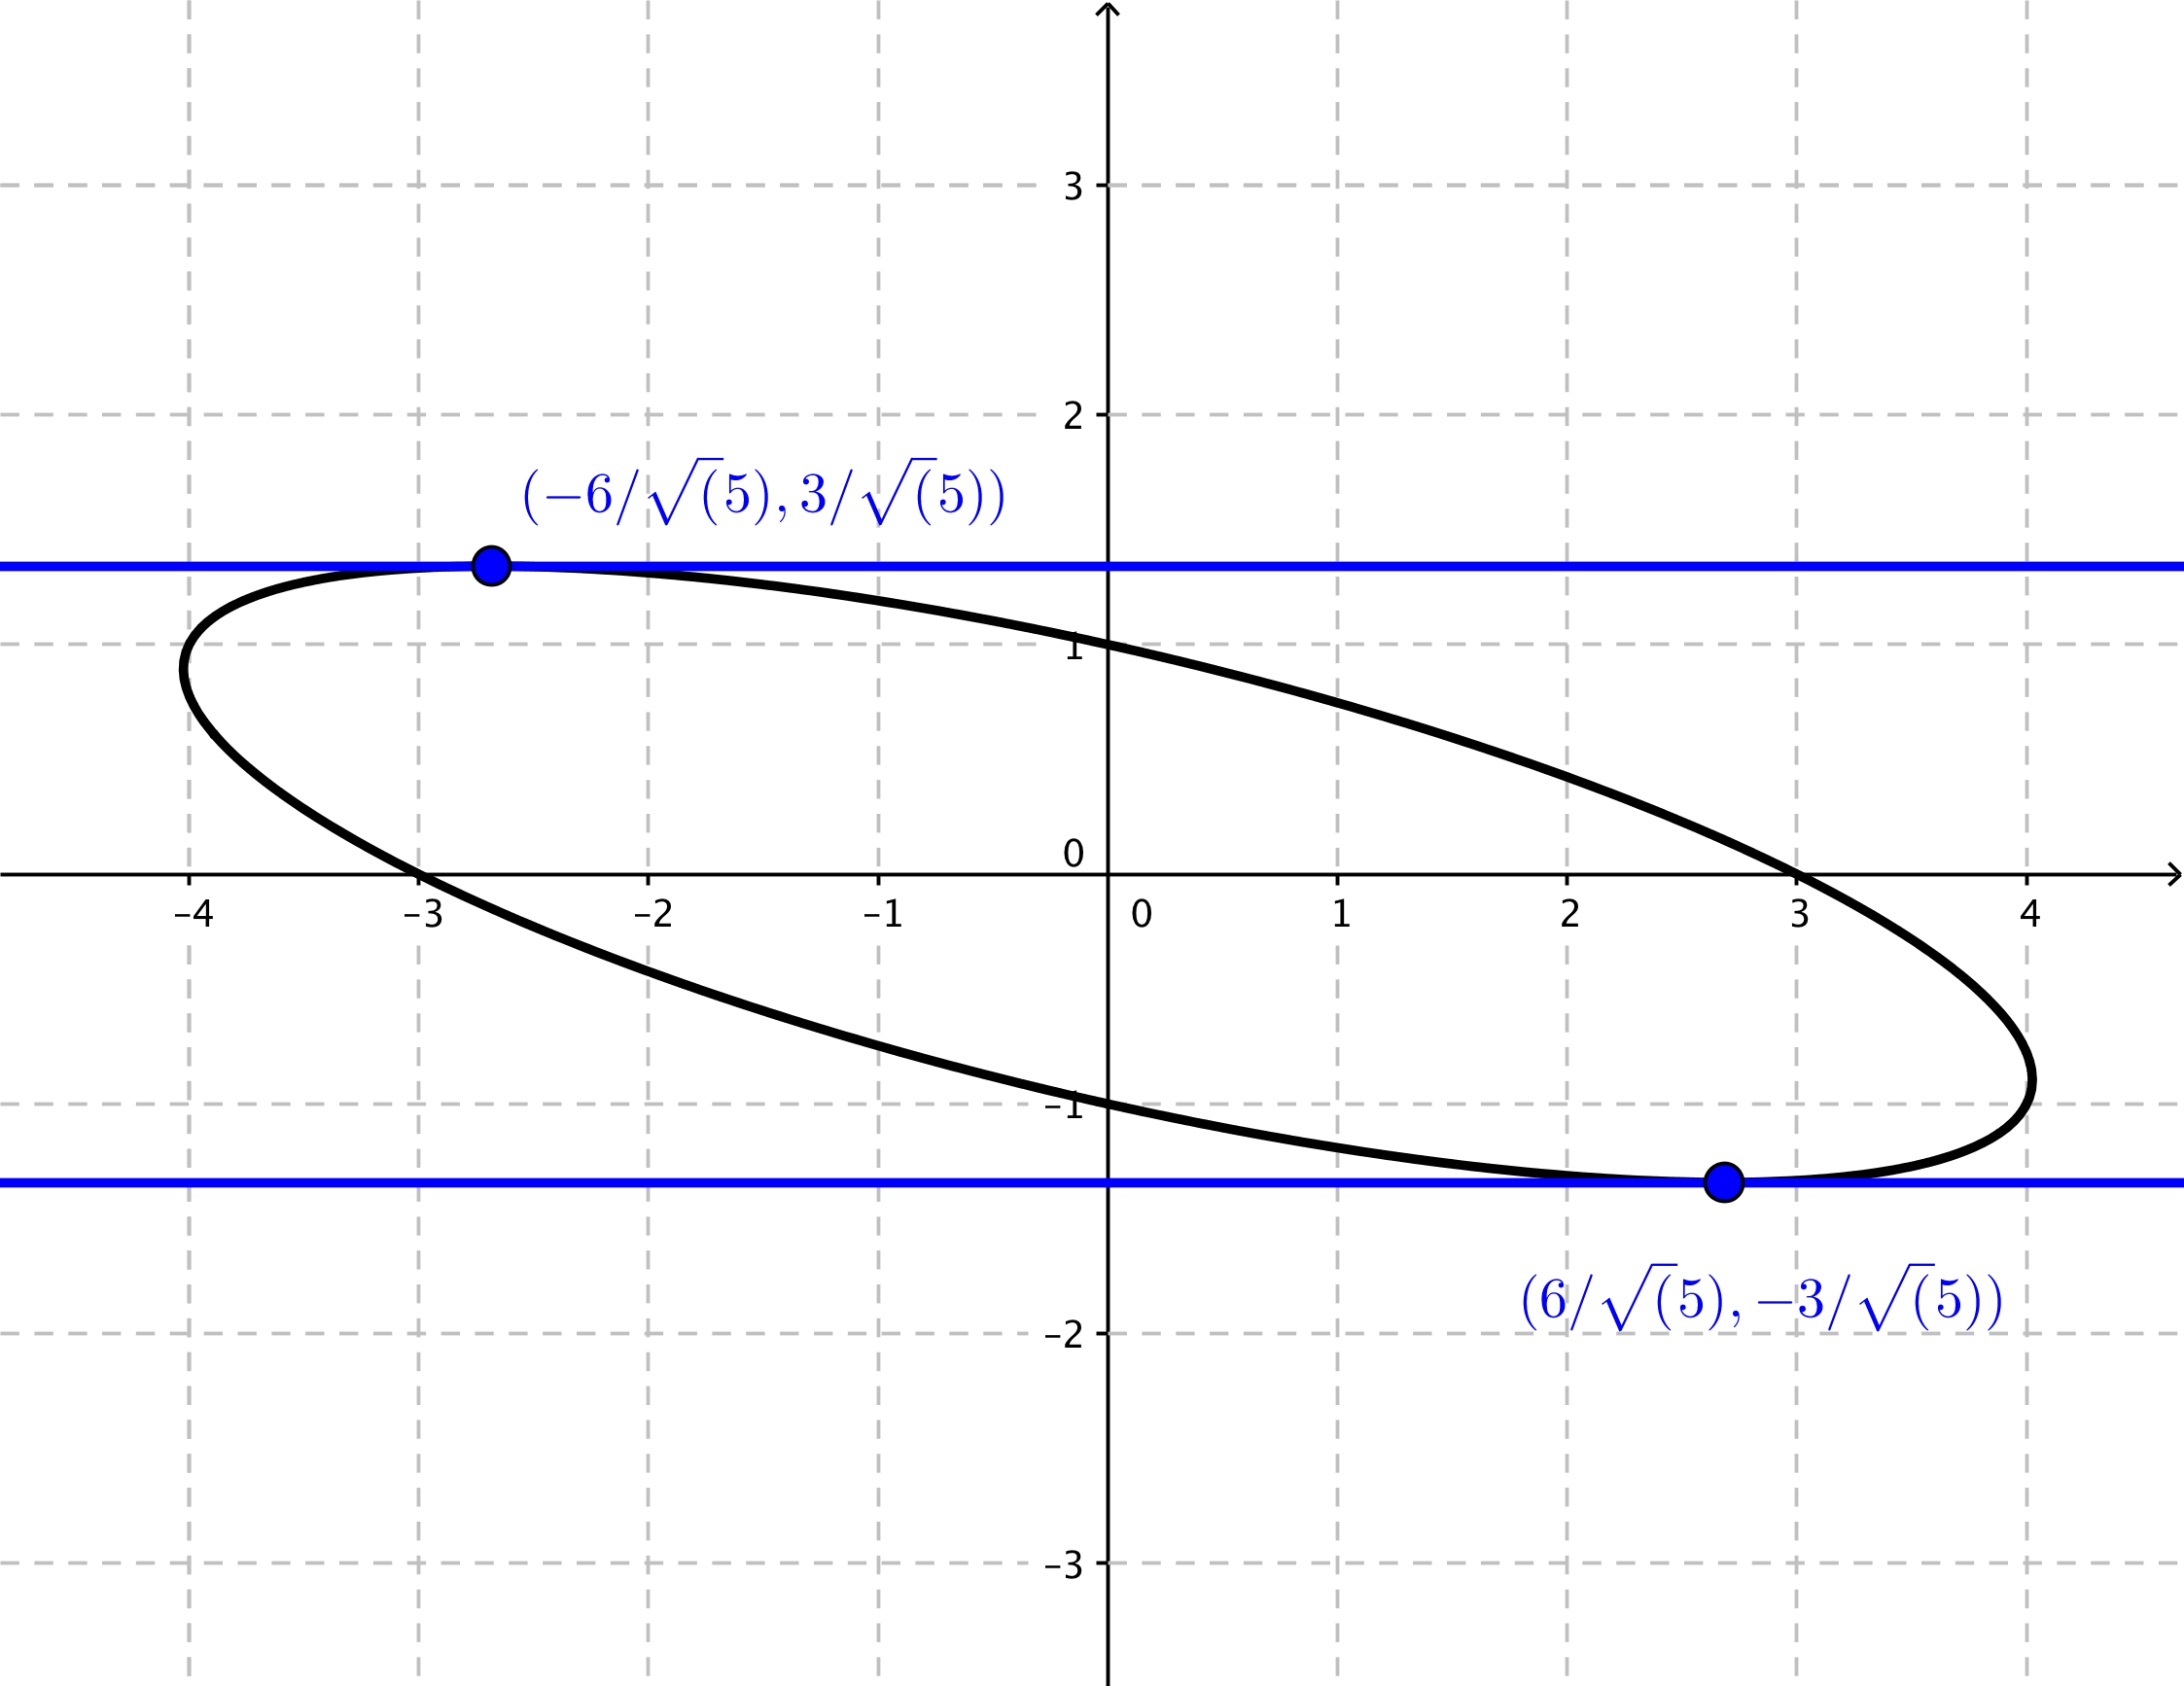
\includegraphics[scale=.4]{figure3.png}
  \end{image}
		\begin{freeResponse}
		$s(1)=-\cos(\pi)+1=-(-1)+1=2$
		  \begin{image}
    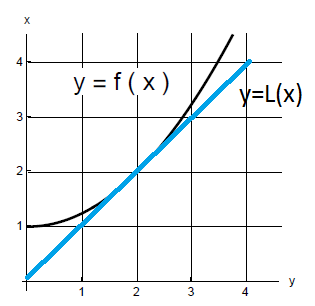
\includegraphics[scale=.4]{figure4.png}
  \end{image}
	\end{freeResponse}
	
	\item Determine the average velocity, $v_{av}$, of the object during the interval $[0,2]$.
	
		\begin{freeResponse}	
	\begin{align*}
	v_{av}&=\frac{s(2)-s(0)}{2-0}\\
	&=\frac{-\cos(2\pi)+1-(-\cos(0)+1)}{2}\\
	&=\frac{-\cos(2\pi)+\cos(0)}{2}\\
	&=\frac{-1+1}{2}=0	
	\end{align*}
	\end{freeResponse}
	
	\item Determine when the motion is in the positive direction.
	
	
	\begin{freeResponse}	
	Motion is in the positive direction when $v(t)>0$.
	
	\begin{align*}
	v(t)>0 & \iff \pi \sin(\pi t)>0\\
	& \iff \sin(\pi t)>0\\
	& \implies 0<\pi t <\pi\\
	& \iff 0<t<1	
	\end{align*}
	\end{freeResponse}
	

	\item At what time (or times) is the object farthest from the origin?

	\begin{freeResponse}	
	Object is farthest from the origin when $\mid{s(t)-0}\mid=\mid{1-\cos(\pi t)}\mid$ is maximized.  Since $s(t) \ge t$ for $t$ in $[0,2]$ we need to maximize $s(t)$.
	Finding critical points on the open interval $(0,2)$.
	\begin{align*}
	v(t)=0 &\iff \pi\sin(\pi t)=0\\
	&\implies \pi t=\pi\\
	&\iff t=1
	\end{align*}
	Finding the absolute maximum, we have to check the endpoints and the critical points:
	\begin{align*}
	s(0)&=0\\
	s(1)&=2\\
	s(2)&=0
	\end{align*}
	Hence the object is farthest from the origin at $t=1$.
	
	\end{freeResponse}



\end{enumerate}

\end{problem}



\end{document} 


















